\documentclass[14pt]{article}
\usepackage[letterpaper, margin=0.6in]{geometry}
\usepackage{fancyhdr}
\usepackage{setspace}
\usepackage{graphicx}
\usepackage{tabularx}
\usepackage{longtable}
\graphicspath{ {/Users/jordanianjoker/Desktop/Rice Programs/} }
\pagestyle{fancy}
\lhead{Ibrahim Al-Akash\\
Sid Richardson}
\rhead{Rice Courseplan}
\lfoot{Class of 2025}
\rfoot{Rice University}
 
\author{\vspace{-5ex}}
\date{\vspace{-5ex}}
\title{\vspace{-5ex}}
\usepackage{lipsum}
\usepackage{changepage}
\usepackage{hanging}
\usepackage{multirow}
\usepackage{amssymb}
\usepackage{marvosym}
 
\singlespacing
 
\begin{document}
\maketitle
\thispagestyle{fancy}
 
 
\begin{center}
    \textbf{Degrees and Courses}\\
    \vspace{1em}
    \def\x{
    \renewcommand*{\arraystretch}{1.6}
    \begin{longtable}{|| p{3.5cm} | c | c | c | c | c | c | c ||}
    \hline
    \multicolumn{8}{|| c ||}{}\\
    \multicolumn{8}{|| c ||}{\emph{Undergraduate Courses}}\\
    \multicolumn{8}{|| c ||}{}\\
    \hline
    \multicolumn{1}{|| c }{Course} & \multicolumn{1}{| c |}{Code} & \multicolumn{4}{ c |}{Description} & \multicolumn{1}{ c |}{Hours} & \multicolumn{1}{ c ||}{Dist Group}\\
    \hline

    INTRODUCTORY BIOLOGY I & BIOS 201 & \multicolumn{4}{p{6cm}|}{The first in a series of two introductory biology courses (BIOS 201, BIOS 202). This course examines chemistry and energetics, cell physiology, cell biology, Mendelian genetics, molecular genetics, developmental biology, and plant physiology.} & 3 & 3\\
	CELL BIOLOGY & BIOS 341 & \multicolumn{4}{p{6cm}|}{Molecular mechanisms of eukaryotic cell function. Structure, function, and biogenesis of all subcellular organelles. Cell-cell communication, cytoskeleton assembly and function, cell cycle control, and cell-cell adhesions. Emphasis will be on cytoplasmic events; molecular studies of transcription are taught in BIOS 302 and BIOS 344.} & 3 & 3\\
	GENERAL CHEMISTRY I & CHEM 121 & \multicolumn{4}{p{6cm}|}{Introduction of chemical phenomena emphasizing problems and methods in Chemistry.} & 3 & 3\\
	GENERAL CHEMISTRY LABORATORY I & CHEM 123 & \multicolumn{4}{p{6cm}|}{Required laboratory component of CHEM 121.} & 1 & 0\\
	GENERAL CHEMISTRY II & CHEM 122 & \multicolumn{4}{p{6cm}|}{A continuation of CHEM 121.} & 3 & 3\\
	GENERAL CHEMISTRY LABORATORY II & CHEM 124 & \multicolumn{4}{p{6cm}|}{Required laboratory component of CHEM 122.} & 1 & 0\\
	ORGANIC CHEMISTRY I & CHEM 211 & \multicolumn{4}{p{6cm}|}{Organic chemistry of aliphatic and aromatic compounds with emphasis on structure, functional groups, bonding, stereochemistry, and reaction mechanisms.} & 3 & 3\\
	INTRODUCTION TO ENGINEERING COMPUTATION & CAAM 210 & \multicolumn{4}{p{6cm}|}{Modeling, Simulation, and Visualization via MATLAB. Numerical methods: Newton's method in one and several dimensions. Gaussian elimination and optimization. Application to problems in science and engineering. Lectures are held Monday and Wednesdays. In a laboratory component held on Fridays, students work in small groups on computational projects led by a Rice Learning Assistant.} & 3 & 3\\
	ELECTRONIC MEASUREMENT SYSTEMS & ELEC 243 & \multicolumn{4}{p{6cm}|}{The course will give students the skills to design, construct, and assess electronic systems to measure, monitor, and control physical properties and events; spans the areas of circuits, signals, systems, and digital processing. Intended for non-ECE majors.} & 4 & 3\\
	SINGLE VARIABLE CALCULUS I & MATH 101 & \multicolumn{4}{p{6cm}|}{Limits, continuity, differentiation, integration, and the Fundamental Theorem of Calculus.} & 3 & 3\\
	SINGLE VARIABLE CALCULUS II & MATH 102 & \multicolumn{4}{p{6cm}|}{Continuation of MATH 101. Includes further techniques of integration, as well as infinite sequences and series, Taylor polynomials and Taylor series, parametric equations, arc length, polar coordinates, complex numbers, and Fourier polynomials.} & 3 & 3\\
	ORDINARY DIFFERENTIAL EQUATIONS AND LINEAR ALGEBRA & MATH 211 & \multicolumn{4}{p{6cm}|}{Study of ordinary differential equations (e.g., solutions to separable and linear first-order equations and to higher-order linear equations with constant coefficients, the properties of solutions to differential equations, and numerical solution methods) and linear algebra (e.g., vector spaces and solutions to algebraic linear equations, dimension, eigenvalues, and eigenvectors of a matrix), as well as the application of linear algebra to first-order systems of differential equations and the qualitative theory of nonlinear systems and phase portraits.} & 3 & 3\\
	MULTIVARIABLE CALCULUS & MATH 212 & \multicolumn{4}{p{6cm}|}{Calculus of multiple variables. Vectors, partial derivatives and gradients, double and triple integrals, vector fields, line and surface integrals, Green's theorem, Stokes's theorem, and Gauss's theorem.} & 3 & 3\\
	ENGINEERING MECHANICS & MECH 211 & \multicolumn{4}{p{6cm}|}{The study equilibrium of static systems, the dynamics of a particle and particle systems, and rigid-body dynamics.} & 3 & 0\\
	MECHANICS (WITH LAB) & PHYS 101/103 & \multicolumn{4}{p{6cm}|}{A calculus-based introduction to mechanics. Includes classes and lab exercises on kinematics, Newton's Laws, work and energy, conservation laws and rotational motion. Primarily for physical science and engineering students.} & 4 & 3\\
	ELECTRICITY \& MAGNETISM (WITH LAB) & PHYS 102/104 & \multicolumn{4}{p{6cm}|}{A calculus-based introduction to electricity and magnetism. Includes classes and lab exercises on electric and magnetic fields, Maxwell's equations in integral form, and AC and DC circuits. Primarily for physical science and engineering students.} & 4 & 3\\
	BIOENGINEERING FUNDAMENTALS & BIOE 252 &  \multicolumn{4}{p{6cm}|}{Introduction to material, energy, charge, and momentum balances in biological systems. Steady state and transient conservation equations for mass, energy, charge and momentum will be derived and applied using basic mathematical principles, physical laws, stoichiometry, and thermodynamic properties. Problem based learning groups will solve open-ended problems.} & 4 & 0\\
	SYSTEMS PHYSIOLOGY LAB MODULE  & BIOE 320 & \multicolumn{4}{p{6cm}|}{Exploration of physiologic systems through measurement of biologic signals. EEG, ECG, EMG pulmonary function tests, etc. are performed and analyzed. Students will explore physiologic concepts through computer simulations, data collection, and analysis.} & 1 & 0\\
	FUNDAMENTALS OF SYSTEMS PHYSIOLOGY & BIOE 322 & \multicolumn{4}{p{6cm}|}{This course will teach the fundamentals of human physiology from an engineering perspective, with specific focus on the nervous, cardiovascular, respiratory and urinary systems. Lectures, assignments and exams will be quantitative and will introduce engineering principles, such as conservation of mass and energy, controls and system analysis, thermodynamics and mass transport, and apply them to the study of physiologic systems.} & 3 & 3\\
	BIOREACTION ENGINEERING & BIOE 330 & \multicolumn{4}{p{6cm}|}{Application of engineering principles to biological processes. Mathematical and experimental techniques for quantitative descriptions of enzyme kinetics, metabolic and genetic networks, cell growth kinetics, bioreactor design and operation.} & 3 & 0\\
	BIOENGINEERING THERMODYNAMICS & BIOE 332 & \multicolumn{4}{p{6cm}|}{This course provides a mathematically rigorous and quantitative coverage of the fundamentals of thermodynamics with applications drawn from contemporary bioengineering problems. Fundamental topics will include the Zeroth, First and Second Law, Entropy Inequality, Gibbs and Helmholtz Free Energies, The Third Law, Maxwell Relations, chemical potential, equilibrium, phase transitions, solution thermodynamics, protein-ligand binding and statistical mechanics. Advanced topics will include transcription factor-DNA binding, nucleic acid hybridization, translation initiation and genetic circuits. The course will cover the role that thermodynamics plays in molecular engineering and synthetic biology.} & 3 & 0\\
	LABORATORY IN TISSUE CULTURE & BIOE 342 & \multicolumn{4}{p{6cm}|}{Introduction to tissue culture techniques, including cell passage, cell viability, and cell attachment and proliferation assays. Students complete quantitative analysis of their data. Engineering design and applications are featured in graded work.} & 1 & 0\\
	BIOMATERIALS & BIOE 370 & \multicolumn{4}{p{6cm}|}{This course will introduce both basic materials science and biological concepts with an emphasis on application of basic quantitative engineering principles to understanding the interactions between materials and biological systems. Topics covered include chemical structure of biomaterials, physical, mechanical, and surface properties of biomaterials, biomaterial degradation, and biomaterial processing. Additional topics include protein and cell interactions with biomaterials, biomaterial implantation, and acute inflammation, wound healing and the presence of biomaterials immune responses to biomaterials, biomaterials, immune responses to biomaterials, biomaterials and thrombosis, as well as infection, tumorigenesis, and calcification of biomaterials that can collectively apply to design of biomaterials for myriad applications.} & 3 & 0\\
	BIOMECHANICS & BIOE 372 & \multicolumn{4}{p{6cm}|}{This course introduces the fundamental principles of mechanics applied to the analysis and characterization of biological systems. Topics covered include normal and shear stresses, normal and shear strains, mechanical properties of materials, load, deformation, elasticity and elastoplastic behavior. Quantitative analysis of statically determinate and indeterminate structures subjected to tension, compression, torsion and bending will be covered. Additionally, aspects of blood rheology, viscoelasticity, and musculoskeletal mechanics will be addressed.} & 3 & 0\\
	BIOMEDICAL INSTRUMENTATION LAB & BIOE 385 & \multicolumn{4}{p{6cm}|}{Students will gain hands on experience with building biomedical instrumentation circuits and systems. Students will learn the basics of lab view programming and signal analysis.} & 1 & 0\\
	BIOMEDICAL ENGINEERING INSTRUMENTATION & BIOE 383 & \multicolumn{4}{p{6cm}|}{This is an introductory level course on fundamentals of biomedical engineering instrumentation and analysis. Topics include measurement principles; fundamental concepts in electronics including circuit analysis, data acquisition, amplifiers, filters and A/D converters; Fourier analysis; temperature, pressure, and flow measurements in biological systems.} & 3 & 0\\
	NUMERICAL METHODS & BIOE 391 & \multicolumn{4}{p{6cm}|}{Introduction to numerical approximation techniques with bioengineering applications. Topics include error propagation, Taylor's Series expansions curre fitting, roots of equations, optimization numerical differentiation and integration, ordinary differential equations, and partial differential equations. Matlab and other software will be used for solving equations.} & 3 & 0\\
	TRANSPORT PHENOMENA IN BIOENGINEERING & CHBE 420 & \multicolumn{4}{p{6cm}|}{BIOE/CHBE 420 covers transport phenomena as applied to biological systems and biomedical devices. Conservation of momentum and mass equations are first derived and then used to analyze transport of momentum and mass in biology, physiology, and in biomedical devices. This course is designed for senior bioengineering students.} & 3 & 0\\
	STATISTICS FOR BIOENGINEERING & STAT 440 & \multicolumn{4}{p{6cm}|}{Course covers application of statistics to bioengineering. Topics include descriptive statistics, estimation, hypothesis testing, ANOVA, and regression.} & 1 & 0\\
	BIOENGINEERING DESIGN I & BIOE 451 & \multicolumn{4}{p{6cm}|}{Senior Bioengineering students will design devices in biotechnology or biomedicine. This project-based course covers systematic design processes, engineering economics, FDA requirements, safety, engineering ethics, design failures, research design, intellectual property rights, environmental impact, business planning and marketing. Students will be expected to compile documentation and present orally progress of their teams.} & 4 & 0\\
	BIOENGINEERING DESIGN II & BIOE 452 & \multicolumn{4}{p{6cm}|}{Senior Bioengineering students will design devices in biotechnology or biomedicine. This project-based course covers systematic design processes, engineering economics, FDA requirements, safety, engineering ethics, design failures, research design, intellectual property rights, environmental impact, business planning and marketing. Students will be expected to compile documentation and present orally progress of their teams.} & 3 & 0\\
	COMPUTATIONAL MODELING LAB & BIOE 446 & \multicolumn{4}{p{6cm}|}{This course offers a hands-on application to systems biology modeling. Students will learn a range of modeling methods, and apply them directly in class to current bioengineering problems. Weekly tutorials will be offered, and a laptop is required (or can be loaned). Topics covered include in silico drug delivery and design studies, integrating multiscale models with high-resolution imaging, experimental design vial computer modeling, and patient-specific simulations. Modeling methods include protein-protein interaction networks, biocircuits, stochastic differential equations, agent-based modeling, computational fluid dynamics, and finite element modeling.} & 2 & 0\\
	DIGITAL DESIGN \& VISUALIZATION & BIOE 447 & \multicolumn{4}{p{6cm}|}{Students will acquire basic to intermediate-level digital design proficiency for bioengineering-related applications. Programs for the design of patient-specific therapies including image reconstruction, computer aided design, and parameter modeling will be used to create models.} & 2 & 0\\
	MICROCONTROLLER APPLICATONS & BIOE 421 & \multicolumn{4}{p{6cm}|}{This class covers the usage of microcontrollers in a laboratory setting. We will start with basic electronics and, in the lab component, design, program, and build systems utilizing widely-available microcontrollers (e.g. Arduino, Raspberry Pi). Units in motion control, sensors (light, temperature, humidity, UV/Vis absorbance), and actuation (pneumatics, gears, and motors) will provide students with functional knowledge to design and prototype their own experimental systems for laboratory-scale automation.} & 3 & 0\\
	IMPLEMENTATION OF DIGITAL SYSTEMS & ELEC 327 & \multicolumn{4}{p{6cm}|}{Embedded microsystems are widely employed to provide intelligence to sensors and actuators throughout our daily life. In this course, we learn the software and hardware frameworks which underly embedded systems design. Students will learn the fundamentals of embedded system programming and feel competent to design, build, and manufacture their own embedded devices. In particular, we focus on principles of low-power design and interface with external peripherals. In addition, students will learn how to design their own manufacturable hardware and discover how application-specific blocks enable modern commercial devices to function. There are weekly lab assignments and two projects.} & 3 & 0\\
	DIGITAL LOGIC DESIGN & ELEC 326 & \multicolumn{4}{p{6cm}|}{Study of gates, flip-flops, combinational and sequential switching circuits, registers, logical and arithmetic operations, introduction to the Verilog hardware description language.} & 3 & 0\\
	INTRODUCTION TO NEUROENGINEERING: MEASURING AND MANIPULATING NEURAL ACTIVITY & BIOE 380 & \multicolumn{4}{p{6cm}|}{This course will serve as an introduction to quantitative modeling of neural activity and the methods used to stimulate and record brain activity.} & 3 & 0\\
	FUNDAMENTALS OF MEDICAL IMAGING I & BIOE 485 & \multicolumn{4}{p{6cm}|}{This course will introduce basic principles of image acquisition, formation and processing of several medical imaging modalities such as X-Ray, CT, MRI, and US that are used to evaluate the human anatomy. The course also includes visits to a clinical site to gain experience with the various imaging modalities covered in class.} & 3 & 0\\
	MATRIX ANALYSIS & CAAM 335 & \multicolumn{4}{p{6cm}|}{Equilibria and the solution of linear systems and linear least squares problems. Eigenvalue problem and its application to solve dynamical systems. Singular value decomposition and its application.} & 3 & 0\\
	CELLULAR ENGINEERING & BIOE 321 & \multicolumn{4}{p{6cm}|}{Introduction to engineering principles and modeling regulation and circuitry at the cellular level. Topics include genetic metabolic networks and cell surface interactions.} & 3 & 0\\
	SENSORY NEUROENGINEERING & BIOE 492 & \multicolumn{4}{p{6cm}|}{This course will explore how bioengineering techniques and principles are applied to understand and model sensory systems, with a focus on the auditory, vestibular, and visual systems. The interaction between the electrical, mechanical and optical aspects of these systems, and ways to modulate these interactions, will be explored. The course will also cover the design of current auditory, visual and somato-sensory neuroprosthetics (i.e. cochlear implants, retinal implants and brain-machine interfaces), as well as emerging technologies for neural stimulation.} & 3 & 0\\
	BIOMATERIALS APPLICATIONS & BIOE 431 & \multicolumn{4}{p{6cm}|}{Emphasis will be placed on issues regarding the design, synthesis, evaluation, regulation and clinical translation of biomaterials for specific applications. An overview of significant biomaterials engineering applications will be given, including topics such as ophthalmologic, orthopedic, cardiovascular and drug delivery applications, with attention to specific case studies. Regulatory issues concerning biomaterial will also be addressed. Assignments for this class will include frequent readings of the scientific literature with occasional homework questions, one midterm and cumulative final, a group project, a seminar report and individual presentations.} & 3 & 0\\
	INTRODUCTION TO ENERGY-EFFICIENT MECHATRONICS & MECH 435 & \multicolumn{4}{p{6cm}|}{Introduction to electromechanical systems, focusing on motor mechanics, electric drives \& electronics, \& modern digital control algorithms. Covers basic principles of electromechanical energy conversion \& motor control. Students are introduced to energy efficiency considerations of modern electric drives. Includes hands-on laboratory projects involving digital computer control of various motor types.} & 3 & 0\\
	DESIGN OF MECHATRONIC SYSTEMS & MECH 488 & \multicolumn{4}{p{6cm}|}{Analog electronic design for purposes of controlling electromechanical systems, including electromechanical sensors and actuators, analog electronic design of filters, state space and classical controllers, and transistor-based servo amplifiers and high voltage amplifiers. Implementation of digital controllers. Significant laboratory component with design and fabrication of circuits to control electromechanical systems.} & 3 & 0\\
	ADVANCES IN BIONANOTECHNOLOGY & BIOE 403 & \multicolumn{4}{p{6cm}|}{This course covers nanotechnology applications in bioengineering. Students learn about cutting edge research that uses the tools of nanotechnology to tackle medical problems. Topics include bionanotechnology - related research for diagnosis, detection, and treatment of disease; cell targeting; drug design and delivery; gene therapy; prostheses and implants and tissue regeneration.} & 3 & 0\\
	NEURO-MUSCULO-SKELETAL MODELING AND SIMULATION & MECH 497 & \multicolumn{4}{p{6cm}|}{Introduction to computer modeling and simulation of the human neuromusculoskeletal system. Topics include measurement of human movement, 3D kinematic modeling, inverse and forward dynamic simulations, muscle and joint contact force estimation, and neural control modeling. Programming proficiency in Matlab required.} & 3 & 0\\
	INTRODUCTION TO ENGINEERING DESIGN AND COMMUNICATION & FWIS 188 & \multicolumn{4}{p{6cm}|}{Students learn the engineering design process to solve real-world problems by evaluating design requirements and constructing innovative solutions in the OEDK. Several communication assignments will be completed by individuals rather than teams.} & 3 & 1\\
	THIRD YEAR ARABIC 1 & ARAB 301 & \multicolumn{4}{p{6cm}|}{Emphasis on developing reading and writing ability as more authentic materials and socio-cultural topics are introduced.} & 3 & 1\\
	THIRD YEAR ARABIC 2 & ARAB 302 & \multicolumn{4}{p{6cm}|}{Emphasis on developing reading and writing ability as more authentic materials and socio-cultural topics are introduced.} & 3 & 1\\
	INTRO TO PSYCHOLOGY & PSYCH 101 & \multicolumn{4}{p{6cm}|}{Survey of topics, problems, and approaches in contemporary psychology. Includes the biological basis of behavior, sensation, perception, attention, learning and memory, thinking, language, abnormal behavior and therapies, personality, and individual differences.} & 3 & 2\\
	DATA, ETHICS, AND SOCIETY & DSCI 305 & \multicolumn{4}{p{6cm}|}{An examination of the ethical implications and societal impacts of choices made by data science professionals. The course will provide practical guidance on evaluating ethical concerns, identifying the potential for harm, and applying best practices to protect privacy, design responsible algorithms, and increase the societal benefit of data science research.} & 3 & 2\\
	PROBABILITY AND STATISTICS FOR DATA SCIENCE & STAT 315 & \multicolumn{4}{p{6cm}|}{An introduction to mathematical statistics and computation for applications to data science. Topics include probability, random variables expectation, sampling distributions, estimation, confidence intervals, hypothesis testing and regression. A weekly lab will cover the statistical package, R, and data projects.} & 4 & 3\\
	INTRODUCTION TO DATA SCIENCE TOOLS AND MODELS & DSCI 302 & \multicolumn{4}{p{6cm}|}{This course introduces key concepts in data management, preparation, and modeling and provides students with hands-on experience in performing these tasks using modern tools, including relational databases and Spark. Models covered include linear and logistic regression and gradient descent.} & 3 & 0\\
	MACHINE LEARNING FOR DATA SCIENCE & DSCI 303 & \multicolumn{4}{p{6cm}|}{This course is an introduction to concepts, methods, best practices, and theoretical foundations of machine learning. Topics covered include regression, classification, kernels, dimensionality reduction, clustering, decision trees, ensemble learning, regularization, learning theory, and neural networks.} & 3 & 0\\
	INTRODUCTION TO EFFECTIVE DATA VISUALIZATION & DSCI 304 & \multicolumn{4}{p{6cm}|}{This course teaches fundamental data visualization skills to undergraduate students in the Data Science minor. Students will learn how to create data visualizations in Python or R, how to design effective visualizations that account for visual perception, and how to explain and present data to technical and non-technical audiences.} & 3 & 0\\
	APPLIED MACHINE LEARNING AND DATA SCIENCE PROJECTS & COMP 449 & \multicolumn{4}{p{6cm}|}{In this project-based course, student teams will complete semester-long data science research or analysis projects selected from a variety of disciplines and industries. Students will also learn best practices in data science.} & 3 & 0\\
	FINANCIAL MANAGEMENT & BUSI 343 & \multicolumn{4}{p{6cm}|}{Develops the core concepts of corporate financial management and introduces a set of analytical tools to evaluate financial decisions. Employs concepts of time value of money, risk and return, and market efficiency are to examine how capital market investors value risky assets. Develops a framework for evaluating corporate investment and financing decisions.} & 3 & 2\\
	INTRODUCTION TO SOCCER & LPAP 125 & \multicolumn{4}{p{6cm}|}{This is an entry level course offering fundamental soccer skills, basic rules, and team tactics. These basic principles will be presented through active participation and instruction and evaluated through physical performance, participation and written assessment.} & 1 & 0\\
	ENTREPRENEURIAL STRATEGY & BUSI 463 & \multicolumn{4}{p{6cm}|}{The first half of this course provides an integrated strategy framework for entrepreneurs. The course is structured to provide a deep understanding of the core strategic challenges facing start-up innovators, and a synthetic framework for choosing and implementing entrepreneurial strategy in dynamic environments, as well as a general understanding of the financing options for early stage startups, including angel investment, accelerators, crowdfunding and the venture capital industry. The course identifies the types of choices that entrepreneurs must make to take advantage of a novel opportunity and the logic of particular strategic commitments and positions that allow entrepreneurs to establish competitive advantage. The second half of the course explores common dilemmas faced by founders surrounding team selection, contracting, equity compensation and incentives, communication in teams, and strategies for approaching each of these dilemmas. The course combines interactive lectures, speakers and case analyses. The cases and assignments offer an opportunity to integrate and apply the principles taught in the course in a practical way, and draws from a diverse range of industries and settings.} & 3 & 0\\

    \hline
    \multicolumn{8}{|| c ||}{Summary}\\
    \hline
    \multicolumn{8}{|| c || }{Total Hours: 167}\\
    \hline
    \multicolumn{2}{|| c |}{Distribution Requirements} & \multicolumn{2}{c}{D1: 9 Hours} & \multicolumn{2}{c}{D2: 9 Hours} & \multicolumn{2}{c ||}{D3: 49 Hours}\\
    \hline
    \multicolumn{8}{|| c ||}{Course Levels}\\
    \multicolumn{2}{|| c}{Level 100: 29 Hours} & \multicolumn{2}{c}{Level 200: 35 Hours} & \multicolumn{2}{c}{Level 300: 58 Hours} & \multicolumn{2}{c ||}{Level 400: 45 Hours}

    \hline
\end{longtable}
}

\def\y{
    \renewcommand*{\arraystretch}{1.6}
    \begin{longtable}{|| p{3.5cm} | c | c | c | c | c | c | c ||}
    \hline
    \multicolumn{8}{|| c ||}{}\\
    \multicolumn{8}{|| c ||}{\emph{Graduate Courses}}\\
    \multicolumn{8}{|| c ||}{}\\
    \hline
    \multicolumn{1}{|| c }{Course} & \multicolumn{1}{| c |}{Code} & \multicolumn{4}{ c |}{Description} & \multicolumn{1}{ c |}{Hours} & \multicolumn{1}{ c ||}{Dist Group}\\
    \hline

	HEALTHCARE INNOVATION AND ENTREPRENEURSHIP & BIOE 527 & \multicolumn{4}{p{6cm}|}{This course is designed for healthcare entrepreneurs who want to build innovative medical technologies. During the course, students will learn how to identify customers, key stakeholders, and the market opportunity for a clinical need; apply design thinking, including low-fidelity prototyping, to quickly test and iterate on a concept; assess regulatory, reimbursement, and clinical trial requirements; identify key assumptions and develop a business model; create a financial model based on business model assumptions; determine capital requirements and funding sources for their venture; understand and evaluate term sheets; create a pitch presentation for investors.} & 3 & 0\\
	HEALTHCARE INNOVATION AND ENTREPRENEURSHIP LAB & BIOE 529 & \multicolumn{4}{p{6cm}|}{In this follow-on experiential Lab course, students work on refining and completing the plan for the venture they created in Health Innovation and Entrepreneurship. Teams receive guidance and Mentoring from faculty and mentors to develop the next steps of their business. The Lab takes place in the Liu Idea Lab for Innovation and Entrepreneurship, a purpose built state-of-the-art incubator and co-working space on the Rice campus.} & 3 & 0\\
	MEDICAL ENGINEERING AND DESIGN LAB & BIOE 528 & \multicolumn{4}{p{6cm}|}{In this studio-based lab, students apply technical engineering and prototyping skills to medical design projects. Participants are taught and apply a range of topics including engineering design processes, medical materials, biocompatibility, design for manufacturing, rapid prototyping, medical equipment, sterility, manufacturing techniques, and quality system implementation.} & 3 & 0\\
	MEDICAL ENGINEERING AND DESIGN LAB 2 & BIOE 530 & \multicolumn{4}{p{6cm}|}{In this studio-based lab, students apply technical engineering and prototyping skills to medical design projects. Participants are taught and apply a range of topics including engineering design processes, medical materials, biocompatibility, design for manufacturing, rapid prototyping, medical equipment, sterility, manufacturing techniques, and quality system implementation. This course is intended for only those students in Bioengineering.} & 3 & 0\\
	MEDICAL INNOVATION INDUSTRY SEMINAR & BIOE 627 & \multicolumn{4}{p{6cm}|}{This course exposes participants to the wide variety of career paths in the medical technology industry including large to mid sized companies, consulting, biotech, pharma, diagnostics, hospital administration and more through guest lectures, case studies, and informational interviews. Additional topics include: Resume and LinkedIn refinement, Job Application Process, Interview Skills, Delivering Oral Presentations} & 1 & 0\\
	ROLES OF PHYSICIANS, SCIENTISTS, ENGINEERS AND MBA'S IN HIGH-TECH STARTUPS & MGMT 633 & \multicolumn{4}{p{6cm}|}{This pragmatic course combines core lectures on entrepreneurship with special guest presentations by notable life science entrepreneurs. It explores the roles that physicians, scientists, engineers, and MBA's play in biotech, medical device, and healthcare companies, as well as major trends in Angel and Venture Capital Financings of Startups. Lectures on entrepreneurial team building, leadership and career planning are included.} & 1 & 0\\
	GRADUATE INDEPENDENT STUDY & BIOE 506 & \multicolumn{4}{p{6cm}|}{Independent investigation of a specific topic in modern bioengineering research under the direction of a faculty member.} & 6 & 0\\
	MANAGEMENT FOR SCIENCE AND ENGINEERING & ENGI 610 & \multicolumn{4}{p{6cm}|}{This course is for graduate and undergraduate students who want to understand the basics of management in new and/or small technology-based businesses and is particularly relevant to students who are interested in careers in technology or entrepreneurial ventures. NSCI 610/ENGI 610 is team taught to provide insight into how technology oriented firms manage people, projects, accounting, marketing, strategy, intellectual property, organizations and entrepreneurship.} & 3 & 0\\
	APPLIED STATISTICS FOR BIOENGINEERING AND BIOTECHNOLOGY & BIOE 539 & \multicolumn{4}{p{6cm}|}{Course will cover fundamentals of probability and statistics with emphasis on application to biomedical problems and experimental design. Recommended for students pursuing careers in medicine or biotechnology.} & 3 & 0\\
	MACHINE LEARNING AND SIGNAL PROCESSING FOR NEURO ENGINEERING & BIE 548 & \multicolumn{4}{p{6cm}|}{The activity of a complex network of billions of interconnected neurons underlies our ability to sense, represent and store the details of experienced life, and enables us to interact with our environment and other organisms. Modern neuroscience techniques enable us to access this activity, and thus to begin to understand the processes whereby individual neurons enable complex behaviors. In order to increase this understanding and to design biomedical systems which might therapeutically interact with neural circuits, advanced statistical signal processing and machine learning approaches are required. This class will cover a range of techniques and their application to basic neuroscience and neural interfaces. Topics include latent variable models, point processes, Bayesian inference, dimensionality reduction, dynamical systems, and spectral analysis. Neuroscience applications include modeling neural firing rates, spike sorting, decoding, characterization of neural systems, and field potential analysis.} & 3 & 0\\
	BUILDING LIFE SCIENCES, BIOMEDICAL AND BIOTECHNOLOGY STARTUPS & BIOE 593 & \multicolumn{4}{p{6cm}|}{This semester-long course aims to provide entrepreneurial students with a hands-on experience in building a high-tech company based on novel biomedical technologies being developed at Rice University and in the Texas Medical Center. Students will form teams of 2-4, and identify a promising biomedical technology, perform intellectual property landscape analysis, identify a minimum viable product, build a business plan, construct 1 year and 5 year financial projections, conduct voice of customer interviews, and present a fundraising ``pitch.'' Students are expected to spend 8-10 hours per week outside the classroom to complete tasks assigned during lectures, and will summarize their findings every 2 weeks in a 7-minute presentation.} & 3 & 0\\
	ENGINEERING DRUG DELIVERY SYSTEMS & BIOE 515 & \multicolumn{4}{p{6cm}|}{This course will focus on the application of innovative engineering approaches to enhance drug efficacy and/or reduce toxicity. Topics of emphasis include, but are not limited to, routes of administration, bioavailability, biodistribution, pharmacokinetics, pharmacodynamics, therapeutic drug windows, patient compliance, immunogenicity, the foreign body reaction, and solubility enhancement. A wide array of device types will be discussed, such as biodegradable microspheres, self-assembled lipid nanoparticles, microneedles, and osmotic pumps. Students will be expected to quantitatively evaluate drug release from complex devices and determine drug distribution and clearance using multi-compartment models. An additional project will be required of graduate level students.} & 3 & 0\\
	NANO-BIOENGINEERING AND NANO-MEDICINE & BIOE 525 & \multicolumn{4}{p{6cm}|}{Covers broad range of topics in nanobioengineering and nanomedicine, including synthesis characterization and fractionalization of nanomaterials and nanostructures, nanoparticle-based molecular imaging probes, nanocarriers, for drug/gene delivery, and nanomachines for gene editing and regulation. Examples will be given to illustrate the applications of nanobioengineering and nanomedicine.} & 3 & 0\\
	ADVANCES IN GENOME EDITING AND ENGINEERING & BIOE 526 & \multicolumn{4}{p{6cm}|}{This is a course for graduate students who are interested in learning the emerging field of precision genome editing and its applications in biology and medicine. This is a lecture course consisting of classes that meet weekly for 3 hours; instruction is delivered both in a lecture setting and through projects.} & 3 & 0\\
	FRONTIERS IN IMMUNO-ENGINEERING & BIOE 536 & \multicolumn{4}{p{6cm}|}{This course will introduce immunology concepts from an engineering perspective and covers various immune responses including to pathogens, self, allergens, cancer, and biomaterials. Using principles of engineering we will perform an in-depth analysis of these responses and the latest advances on the development of novel therapeutics. Topics include systems immunology, nanotechnology, hydrogels, biomaterials, vaccines, cancer immunotherapy, autoimmunity, tissue engineering, stem cells, viruses, and the microbiome.} & 3 & 0\\
	3D PRINTING AND ADDITIVE MANUFACTURING: THEORY AND APPLICATIONS & MSNE 513 & \multicolumn{4}{p{6cm}|}{Basic principles and applications of additive manufacturing (AM), Various AM processes. Materials science such as polymers, metals, ceramics, composites, and bio-materials for AM. Selection of material and process for design applications such as structures, electronics, biomedical, and consumer products. Hands-on experience and analysis from digital data to physical objects.} & 3 & 0\\

    \hline
    \multicolumn{8}{|| c ||}{Summary}\\
    \hline
    \multicolumn{8}{|| c || }{Total Hours: 48}\\
    \hline
    \multicolumn{8}{|| c ||}{Course Levels}\\
    \multicolumn{2}{|| c}{Level 400: 0 Hours} & \multicolumn{2}{c}{Level 500: 42 Hours} & \multicolumn{2}{c}{Level 600: 6 Hours} & \multicolumn{2}{c ||}{Other: 0 Hours}

    \hline
\end{longtable}
}

\x

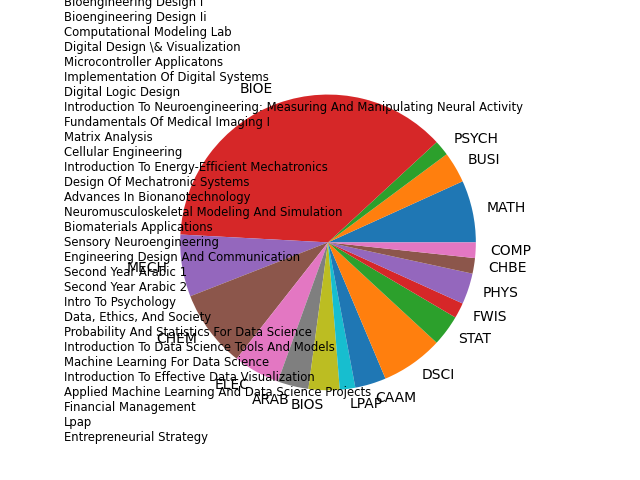
\includegraphics[scale=0.6]{Undergrad Course Pie.png}

\y

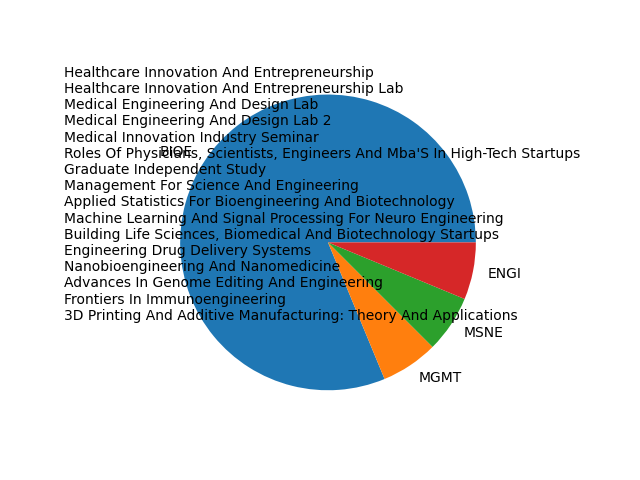
\includegraphics[scale=0.6]{Grad Course Pie.png}

\end{center}


 
\end{document}